% Chapter X

\chapter{Majorana Interlude} % Chapter title

\label{ch:majinter} % For referencing the chapter elsewhere, use \autoref{ch:dsmcehr} 

%----------------------------------------------------------------------------------------

\begin{flushright}{\slshape    
It's very hard to talk quantum\\
using a language originally designed\\
to tell other monkeys where the ripe fruit is.} \\ \medskip
--- Terry Pratchett, Night Watch
\end{flushright}

\bigskip

%-----------------------------------------------------------------------------------------

General scope for the problem.

Inadequacies in alternative approaches. Should mention some of the full quantum models of the Stern Gerlach problem ie: Sukmar and Brink etc.

Majorana's approach does not require the extension into the imaginary time domain nor does he make dodgey mistakes in an attempt to engineer the solution.

As mentioned in section \autoref{ch:intro} the original experimental realisations of BEC were hindered by the unwanted selective loss of the coldest atoms in the gas cloud \cite{Cornell2002, Ketterle2002}.
This loss, it was found, was caused by non-adiabatic spin transitions of atoms close to the minimum of the magnetic trapping potential.

Papers I should reference in this introduction are \cite{Bloch1945,Giacomo2005,Wittig2005,Ma2006, Vutha2010}.

The print history of the Majorana solution is a little funny.
Originally printed in il nuova cimento in 1932 \cite{Majorana1932-orig} it was subsequently translated and reprinted in Societ\'a Italiana di Fisica in 19?? \cite{?}.
Unfortunately both the original and the reprint contain some small typographical errors that may make it difficult for readers to follow.
In an attempt to remedy this problem, as well as elucidate the complex asymptotic method Majorana used in his solution, the following sections will outline, in excruciating detail, the correct solution -- error free.
Readers may also find this a useful introduction to, and a practical application of, the method of steepest descents.

%-----------------------------------------------------------------------------------------

\section{Derivation of the Differential Equation}

To illustrate the theory of an avoided crossing we will consider the case of a static 2-level atom in a dynamic field. 
The interaction Hamiltonian for a magnetic dipole in a magnetic field is $\widehat{H}_{B} = -\hat{\boldsymbol{\mu}} \cdot \boldsymbol{B}$, written in matrix form is
\begin{equation}
	\widehat{H}_{B} = \hbar \gamma \begin{bmatrix} B_{z} & B_{x} - i B_{y}\\
											B_{x} + i B_{y} & -B_{z} \end{bmatrix}, \label{Eq:MagHam}
\end{equation}
where $\gamma = g_{F}\mu_{B}M_{F} / \hbar$ is the gyromagnetic ratio and represents the proportionality between the spin and magnetic moment, $\hat{\boldsymbol{\mu}}$, operators. 
If we choose the ``spin up,'' $\vert\uparrow\rangle$ and ``spin down,'' $\vert \downarrow\rangle$ states as our basis then, the diagonal elements are the energies of our basis (or diabatic) states and the off diagonal elements represent the coupling between states. 
The eigenvalues for the hamiltonian in \eqref{Eq:MagHam} are 
\begin{equation}
	E_{\pm} = \pm \hbar \gamma \sqrt{{B_{x}}^{2} + {B_{y}}^{2} + {B_{z}}^{2}},
\end{equation}
and correspond to the states perfectly aligned (and anti-aligned) with the local magnetic field. 
We can see the effect of the coupling between states in these eigen-energies through the appearance of the term, $\left\vert\Delta\right\vert^{2} = {B_{x}}^{2} + {B_{y}}^{2}$. 
More specifically consider the two situations shown in figure \ref{Fig:AvoidedCrossing}. 
When there is no coupling we get the grey curves and when there is coupling we get the coloured curves \textcolor{red}{(explain)}. 
If we consider a time-dependant magnetic field in which the coupling is constant and the diagonal field changes from large and negative to large positive very slowly (or \emph{adiabatically}) then the system should follow the one of the curves. 
If it goes quickly then it might jump across the gap \textcolor{red}{(this is rubbish)}.

The time-dependant magnetic field discussed in Majorana's paper \cite{Majorana1932} is ${\mathbf B} = \left(A, 0 , -Ct\right)$ and so the corresponding coupled time-dependant Schr\"odinger equations for a spin half particle with $\vert\psi(t)\rangle = c_{1}(t) \vert \downarrow\rangle + c_{2}(t) \vert \uparrow \rangle$, are
\begin{subequations}
\begin{align}
	\dot{c_{1}} &= - \gamma i \left(-Ctc_{1} + Ac_{2}\right),\\
	\dot{c_{2}} &= - \gamma i \left(A c_{1} + Ct c_{2}\right).
\end{align}
\end{subequations}
Using the dimensionless time
\begin{equation}
	\tau = \sqrt{\frac{\gamma \, C}{2}} \, t,
\end{equation}
and the numerical quantity
\begin{equation}
	k = \frac{2\gamma A^{2}}{C},
\end{equation}
which describes the ratio of the atom precession frequency to the rotation frequency of the field direction at the field minimum, we can obtain the coupled differential equations
\begin{subequations} \label{eq:Majprob}
\begin{align}
	\frac{dc_{1}}{d\tau} &= - i \left(-2\tau c_{1} + \sqrt{k}c_{2}\right),\\
	\frac{dc_{2}}{d\tau} &= -i \left(\sqrt{k} c_{1} + 2\tau c_{2}\right).
\end{align}
\end{subequations}
These equations can be further simplified through the application of the integration factor method \cite{Kreyszig2006}, by setting
\begin{equation}
	c_{1} = e^{i\tau^{2}}f, \quad \quad
	c_{2} = e^{-i\tau^{2}}g,
\end{equation}
from which it follows
\begin{subequations}
\begin{align}
	\frac{df}{d\tau} &= -i \sqrt{k} e^{-2i\tau^{2}}g,\\
	\frac{dg}{d\tau} &= -i \sqrt{k} e^{2i\tau^{2}}f. \label{Eq:dgdt}
\end{align}
\end{subequations}
Eliminating $g$, we obtain\footnote{The factor of $4i\tau$ was erroneously printed as $hi\tau$.}
\begin{equation}
	\frac{d^{2}f}{d\tau^{2}} + 4 i \tau \frac{df}{d\tau} + kf = 0. \label{Eq:fDiff}
\end{equation}
This differential equation holds the answers we seek. 
It describes the evolution of the probability density of the spin up state of the system.
Thus if we kind find a solution to this equation we will know how the system's spin changes over time.
Even with modern symbolic computation packages like Mathematica, it is very difficult to find a solution to this equation that satisfies the boundary conditions we have.
So, we must seek an asymptotic solution, if we can't know what the spin does for all values of time, maybe we can at least have an idea what the spin is doing at the end of time?
%-----------------------------------------------------------------------------------------

\section{Transforming into an Integral Equation}

When obtaining an asymptotic solution to a differential equation it is often preferable to investigate the asymptotic behaviour of an integral solution. 
It is not always possible to obtain an integral solution, but when possible it provides a global solution from which all asymptotic limits can be obtained, and hence connect solutions from one end of the domain to another\footnote{The alternative of course is to use a local method like perturbation analysis to investigate the local behaviour of the solution.}. 
It is with this motivation that we seek to find an integral representation of \autoref{Eq:fDiff}. 
NOTE: Find the name of the following method with suitable references and motivation.
To this end we will assume the solution can be written as an integral of the product between a given kernel $K(s,\tau)$ and some unknown function\cite{White2005} $\chi(s)$,
\begin{equation}
	f(\tau) = \int_{C} K(s,\tau) \chi(s) \, ds,
\end{equation}
where $C$ is an arbitrary contour in the complex plane and $K$ and $\chi$ are \emph{complex functions} of the \emph{complex variable} $s$. 
Our job now, of course, is to find an expression for $\chi(s)$.
We will use the Fourier Laplace kernel, $K(s,\tau) = e^{s\tau}$, so that the differential \autoref{Eq:fDiff} becomes
\begin{equation}
	\int_{C}\chi(s) \left(s^{2}+k\right)e^{s\tau}\, ds + 4i\int_{C}\chi(s)s\tau e^{s\tau} \, ds = 0.
\end{equation}
Integrating the second term by parts gives
\begin{equation}
	\left.\int_{C}\left[\left(s^{2}+k-4i\right)\chi(s) - 4is \chi'(s)\right] e^{s\tau}\, ds + \textcolor{blue}{s\chi(s)e^{s\tau}}\right\vert_{C} = 0.
\end{equation}
Given that we made no specifications about the contour our arbitrary contour, $C$, we can choose it such that the boundary term, in blue, disappears. 
In general, if an integral over an arbitrary contour is zero we can say that the integrand must also be equal to zero, this gives the differential equation
\begin{equation}
	\left(s^{2}+k-4i\right)\chi(s) - 4is \chi'(s) = 0,
\end{equation}
which is separable and has solution the solution
\begin{equation}
	\chi(s) = As^{(k/4i) - 1}e^{s^{2}/8i},
\end{equation}
so long as $\log s$ assumes its principle value\footnote{i.e. $\log s = \log_e \vert s \vert + \imath \text{Arg}s$.}. 
Here $A$ is a constant of normalisation that will be determined in \autoref{Sec:Asymp}. 
Thus we have 
\begin{equation}
	f(\tau) = A\int_{C}s^{(k/4i)-1}e^{(s^{2}/8i)+s\tau}\, ds, \label{Eq:AsymInt}
\end{equation}
with the boundary condition
\begin{equation}
	\left.s^{k/4i}e^{(s^{2}/8i)+s\tau}\right\vert_{C}=0.
\end{equation}
This boundary condition could be easily satisfied by the rays where $\text{Arg} \,s = -\frac{\pi}{4}, \, \frac{3\pi}{4}$ for example.

%-----------------------------------------------------------------------------------------

\section{Asymptotic Solution of the Integral} \label{Sec:Asymp}

The simplest technique for obtaining the asymptotic behaviour of integrals in which an asymptotically large parameter $\tau$ appears as an exponential
\begin{equation}
	I(\tau) = \int_{a}^{b} h(s) e^{\tau\phi(s)} \, ds,
\end{equation}
is Laplace's method \cite{Bender1999}, where we assume $h(s)$ and $\phi(s)$ are \emph{real} and \emph{continuous}. 
The foundation of Laplace's method is the idea that if the real continuous function $\phi(s)$ has its \emph{maximum} on the interval of integration, $a \le s \le b$, at $t = c$ and if this maximum is not equal to zero, $h(c) \ne 0$, then it is only the \emph{immediate neighbourhood} of $t=c$ that contributes to the full asymptotic expansion of $I(\tau)$ for large $\tau$. 
That is we may approximate the integral $I(\tau)$ by $I(\tau; \epsilon)$ where
\begin{align}
	I(\tau;\epsilon) &= \int_{c-\epsilon}^{c+\epsilon}h(s) e^{\tau\phi(s)}\, ds,\\
	&\approx \int_{c-\epsilon}^{c+\epsilon}\left[h(c) + \left(s-c\right)h'(c) + {\cal O}(s^{2})\right]e^{\tau\left[\phi(c)+\left(s-c\right)\phi'(c) + \frac{1}{2}\left(s-c\right)^{2}\phi''(c)+{\cal O}(s^{3})\right]}\, ds,\\
	&\approx h(c)e^{\tau\phi(c)}\int_{-\infty}^{\infty} e^{\tau\left(s-c\right)^{2}\phi''(s)/2}\, ds, \quad \text{as }\tau \to + \infty. \label{Eq:Laplace}
\end{align}
If we try to apply this to our problem however, we notice straight away that in \autoref{Eq:AsymInt} we have $h(s) = s^{(k/4i)-1}e^{s^{2}/8i}$. This expression isn't real, nor is the variable of integration, thus Laplace's method is not directly applicable.
We will instead, employ a technique known as the method of steepest descents \cite{Bender1999}. 
Analogous to Laplace's method, the method of steepest descents is a technique for finding the asymptotic behaviour of integrals of the form
\begin{equation}
	I(\tau) = \int_{C}h(s) e^{\tau \rho(s)} \, ds, \label{Eq:SteepestDescent}
\end{equation}
where $C$ is an integration contour in the complex $s$ plane and $h(s)$ and $\rho(s)$ are \emph{analytic functions} of $s$. 
Here the idea is to use the analyticity of the integrand to justify deforming the contour $C$ to a new contour $C'$ on which the imaginary part $\rho(s)$ is constant.
Once this has been done, $I(s)$ may be evaluated asymptotically using Laplace's method. 
To see why, observe that on the contour $C'$ we may write $\rho(s) = \phi(s) + i \psi$, where $\psi$ is a real constant and $\phi(s)$ is a real function. 
Thus, $I(s)$ in \autoref{Eq:SteepestDescent} takes the form
\begin{equation}
	I(s) = e^{is\psi} \int_{C'}h(s) e^{\tau\phi(s)}\, ds.
\end{equation}
Again our particular problem is not as straight forward. We cannot simply use $\rho(s) = s$ since it's maximum is infinite. As we expect the integral to be convergent, we instead have to consider the entire exponent $\rho(s) = s^{2}/8i+s\tau$. 
If we plan on using Laplace's method to approximate the integral along the deformed contour then we require that the new contour passes through the stationary point of $\rho(s)$. 
The stationary point of $\rho(s)$ will be at $ s_{\text{st.pt.}} = -4i\tau$. 
Recall that we are looking to deform our contour so that the imaginary part of $\rho(s)$ is constant and equal to it's maximum value, the value at the stationary point, $\psi = \Im(\rho(s_{\text{st.pt}})) = \Im(-4\imath\tau) = -2\tau^{2}$.

To parameterise the deformed contour, $C'$, we let $s = p + iq$ so that  
\begin{equation}
	\rho(s) = \rho(p,q) = \left[\frac{1}{4}pq + \tau p\right] + i \left[ \frac{1}{8}q^{2} - \frac{1}{8}p^{2} + \tau q\right].
\end{equation}
The contours along which the imaginary part of $\rho(s)$ is constant and equal to $\psi=-2\tau^{2}$ are thus given by
\begin{align}
	-2\tau^{2} &= \frac{1}{8}q^{2} + q\tau - \frac{1}{8}p^{2},\\
	\Rightarrow q &= -4\tau \pm p.
\end{align}
These two contours are shown in \autoref{Fig:ContourPlots}. 
Since we require that the stationary point $s_{\text{st.pt.}}=-4i\tau$ be a maximum we will choose the contour $q=-4\tau-p$ so that we now have
\begin{equation}
	s = -4i \tau + \left(1 - i\right)p, \quad ds = \left(1 - i\right) dp. \label{eq:deformed_contour}
\end{equation}
Now that we finally have our contour we can make use of Laplace's method by substituting \autoref{eq:deformed_contour} into \autoref{Eq:AsymInt}
\begin{equation}
	f(\tau) =A\left(1-i\right)e^{-2i\tau^{2}}\int_{-\infty}^{\infty}\left(-4i\tau + \left(1-i\right)p\right)^{(k/4i)-1}e^{-p^{2}/4}\, dp. \label{eq:laplace_f}
\end{equation}
This might not look any more tractable at first glance, but importantly we have removed the asymptotically large parameter, $\tau$, from the exponent, which allow us to derive far more meaningful asymptotic expressions.

We'll begin with the easy case first.
Let's consider the beginning of time, the limit when $\tau \to -\infty$.
While $\tau < 0$ we can solve \autoref{eq:laplace_f} directly to find
\begin{align}
	f(\tau) &\approx A\left(1-i\right)e^{-2i\tau^{2}}\left(-4i \tau\right)^{k/4i-1}\int_{-\infty}^{\infty}e^{-p^{2}/4}\, dp, \quad \text{as } \tau \to -\infty\\
	&= 2A\left(1-i\right)\sqrt{\pi}e^{-2i\tau^{2}}\left(-4i \tau\right)^{k/4i-1}, \quad \text{as } \tau \to -\infty.
\end{align}
In the limit $\tau \to -\infty$ we can see $f(\tau) \to 0$, due mostly to the negative exponential power of $\tau$.
This asymptotic behaviour matches our initial condition, that the system begins in the spin up state.
Using \autoref{Eq:dgdt} to find $g(\tau)$ we have 
\begin{align}
	g(\tau) &= \int_{-\infty}^{\tau}2kAi\left(1-i\right)\sqrt{\pi}\left(-4i \tau' \right)^{k/4i-1}\, d\tau', \quad \text{as } \tau \to -\infty\\
	&= 2A\left(1+i\right)\sqrt{\pi}\left(-4 \tau' \right)^{k/4i}e^{k\pi/8} , \quad \text{as } \tau \to -\infty.
\end{align}
Now since we require that $\left\vert g\right\vert^{2} \to 1$ as $\tau \to - \infty$ to satisfy the initial condition we find that $A = \sqrt{k}e^{-k\pi/8}/(2(1+i)\sqrt{\pi})$.

Now when we consider the end of time, $\tau \to 0$, things get a little trickier.
When describing Laplace's method earlier I stressed the importance of the analyticity of the integrand.
However when $\tau > 0$ the integration contour will have to cross a branch cut along the negative real axis caused by the fractional powers of $s$. 
In this case we will follow the path indicated in figure \ref{Fig:IntegrationPaths}. 
It is easier to evaluate this integral if we split it up into several components.
So now let
\begin{align}
	f(\tau) &= \int_{\gamma_{1}} + \int_{\gamma_{2}} + \int_{\gamma_{3}} + \int_{\gamma_{4}} + \int_{\gamma_{5}},\\
	&= f_{1} + f_{2} + f_{3} + f_{4} + f_{5} .
\end{align}
Now the asymptotically dominant component of the integral will actually come from the branch cut, but I will show the behaviour of each component to be sure.
\textcolor{red}{Can show $f_{1}$ and $f_{3}$ tend to zero (at least in the limit $\tau \to 0$)}. 
Often the contributions from the branch cuts work together, they will either cancel or add providing some sort of symetry that can be exploited in symplification.
With that in mind lets consider the two paths along the branch cut.
Along $\gamma_{2}$ we let $s = pe^{i \pi} = -p$ where $ds = e^{i \pi}dp$, so now \autoref{Eq:AsymInt} becomes
\begin{equation}
	f_{2} = \frac{\sqrt{k} e^{-k\pi/8}}{2\left(1+i\right)\sqrt{\pi}}\int_{-4\tau}^{\epsilon} p^{(k/4i)-1}e^{k\pi/4}e^{(p^{2}/8i) -p\tau}\, dp.
\end{equation}
Similarly along $\gamma_{4}$ we let $s = pe^{-i\pi} = p$ where $ds = e^{-i\pi}dp$ so that
\begin{equation}
	f_{4} = -\frac{\sqrt{k} e^{-k\pi/8}}{2\left(1+i\right)\sqrt{\pi}}\int_{-4\tau}^{\epsilon} p^{(k/4i)-1}e^{-k\pi/4}e^{(p^{2}/8i) -p\tau}\, dp.
\end{equation}
Now adding together $f_{2}$ and $f_{4}$, and making use of a Taylor series expansion we have
\begin{align}
	f_{2} + f_{4} &= \frac{\sqrt{k} e^{-k\pi/8}}{2\left(1+i\right)\sqrt{\pi}}\int_{-4\tau}^{\epsilon} p^{(k/4i)-1}e^{(p^{2}/8i) -p\tau}\left(e^{k\pi/4}-e^{-k\pi/4}\right)\, dp,\\
	&= \frac{\sqrt{k} e^{-k\pi/8}}{\left(1+i\right)\sqrt{\pi}}\sinh\left(\frac{k\pi}{4}\right)\int_{-4\tau}^{\epsilon} p^{(k/4i)-1}e^{(p^{2}/8i) -p\tau}\, dp,\\
	&= \frac{\sqrt{k} e^{-k\pi/8}}{\left(1+i\right)\sqrt{\pi}}\sinh\left(\frac{k\pi}{4}\right)\int_{-4\tau}^{\epsilon} p^{(k/4i)-1}e^{-p\tau}\left(1 + \frac{p^{2}}{8i} + {\cal O}(p^{4})\right)\, dp.
\end{align}
Looking at the above equation it is clear that if we make the substitution $p\tau = p'$ so that $dp = \tau^{-1}dp'$ we have will have (to the highest order in $\tau$) the integral form of the gamma function so that
\begin{equation}
	f_{2}+f_{4} = \frac{\sqrt{k} e^{-k\pi/8}}{\left(1+i\right)\sqrt{\pi}}\sinh\left(\frac{k\pi}{4}\right)\tau^{-k/4i}\Gamma\left(\frac{k}{4i}\right).
\end{equation}
The contributions from $f_1$ and $f_5$ can be found by using Laplace's method.
In $f_5$ the contribution comes from the saddle point at $\tau= -4\imath\tau$ and can be found the same way as for the $\tau < 0$ case so 
\begin{equation}
	f_{5} = -i\sqrt{k}e^{k\pi/8-2i\tau^{2}}\left(-4i \tau\right)^{-1-k/4i}, \quad \text{as } \tau \to \infty.
\end{equation}
The $\gamma_{1}$ contour will follow the same derivation as the $\gamma_{5}$ except that it's maximum is at the $x$-intercept, $x=-4\tau$, so the Taylor series expansion must be made about this maximum. 
Thus we have
\begin{equation}
	f_{1} = -i\sqrt{k}e^{k\pi/8-2i\tau^{2}}\left(-4 \tau\right)^{-1-k/4i}, \quad \text{as } \tau \to \infty.
\end{equation}
Both of these terms will decay exponentially as $\tau \to \infty$, again due to the negative exponential in $\tau$.
This means the only asymptotically non-zero contribution comes from the branch cut.
So finally we have\footnote{The $\tau^{-k/4i}$ was erroneously printed as $e^{-k/4i}$.} in the limit as $\tau \to \infty$
\begin{equation}
	f(\tau) =  \frac{\sqrt{k} e^{-k\pi/8}}{\left(1+i\right)\sqrt{\pi}}\sinh\left(\frac{k\pi}{4}\right)\tau^{-k/4i}\Gamma\left(\frac{k}{4i}\right),
\end{equation}
and 
\begin{equation}
	g(\tau) = (4\tau)^{k/4i}e^{-k\pi/4}.
\end{equation}

%-----------------------------------------------------------------------------------------

\section{Conclusion} \label{sec:majorana_conc}

The probability of the spin adiabatically flipping will be given by 
\begin{equation}
    \left\vert g \right\vert^{2} = e^{-k\pi/2} \textrm{ as } \tau \to \infty. \label{eq:majProb}
\end{equation}
\textcolor{red}{(Explain the changing sign of the magnetic field swaps the basis vectors.)}

\section{Landau Zener Formula}

Content

\section{Loss Rates 'n' Stuff} \label{sec:majorana_loss_rates}

Now that we have the solution to the Majorana problem we can use this formula to derive loss rates for atoms in real trapping potentials.
The following section will outline the work done by Porto \cite{Lin2009,Dubessy2014} in a clear methodical manner, allowing the reader to fully understand the assumptions made when deriving the current loss model.

We begin with the heuristic derivation given by Petrich et al in \cite{Petrich1995}.
In \autoref{sec:majorana_conc} we saw that, very broadly, for an atom to undergo a non-adiabatic spin flip we require that the Larmor precession frequency must be smaller than the rate of change of the magnetic field direction.
The Larmor precession frequency is given by
\begin{equation}
    \omega_{\textrm{L}} = \gamma \vert \mathbf{B}(\mathbf{r}) \vert.
\end{equation}
For an atom passing a minimum distance of $b$, in a trap with a radial gradient $\partial B_r / \partial r = B_q'$, we have $\omega_{\textrm{L}} \sim \gamma B_q' b$. 
We can also, very approximately, estimate the rate of change of the magnetic field direction for an atom moving with a velocity $v$ to be, $\omega_{\mathrm{B}} \sim v / b$ (see \autoref{sec:maj_loss_der} for a more accurate estimate).
Thus we may define the surface of a sphere at which the conditions for a transition are met, with a radius $b_0$
\begin{align}
    \omega_{\textrm{L}} &\approx \omega_{\textrm{B}},\\
    \gamma B_q' b_0 &\approx \frac{v}{b_0},\\
    b_0(v) &\approx \sqrt{\frac{v}{\gamma B_q'}}. \label{eq:majorana_radius}
\end{align}
We can now pick up with the work from Porto, which tries a little harder to eliminate unnecessary assumptions.
So far we can describe the velocity dependant surface through which an atom must travel to undergo a non-adiabtic transition.
To be able to estimate a loss rate we must find the number of atoms flowing through this surface.
The local particle flux through this surface is given by, $j(v) = v n( \mathbf{r}(v),p)$, where $n(\mathbf{r}(v),p)$ is the local atom density. 
As the radius of the above sphere is typically very small, we can make that assumption that local atom density is constant and equal to the central density of the cloud, $n(\mathbf{r}(v),p) \approx n(0,p) = n_0$.
Thus if the flux is constant we can find the number of atoms crossing the surface of the velocity dependant sphere by multiplying the flux by the surface area of the sphere
\begin{align}
    \Gamma_{\textrm{M}}(v)N &= 4\pi C b_0^2(v)j(v),\\ 
    &= \frac{ 4\pi C n_0 v^2 } { \gamma B_q'}.
\end{align}
At this point we have introduced a constant $C$ to account for the approximations we have made above.
This is essentially a geometric factor that will change depending of the shape and structure of the trapping potential.
We can now average this loss rate over all velocities
\begin{align}
    \Gamma_\textrm{M}N &= \frac{ 4\pi C n_0 } { \gamma B_q'} \left< v^2 \right>,\\
    &= \frac{ 4\pi C n_0 } { \gamma B_q'} \frac{ \iiint v^2 e^{-\frac{p^2}{2mk_\textrm{B}T}}\, d^3p}{\iiint e^{-\frac{p^2}{2mk_\textrm{B}T}}\,d^3p},\\
    &= \frac{ 4\pi C n_0 } { \gamma B_q'} \frac{ \int v^4 e^{-\frac{mv^2}{2k_\textrm{B}T}}\, dv}{\int v^2 e^{-\frac{mv^2}{2k_\textrm{B}T}}\,dv},\\
    &= \frac{ 4\pi C n_0 } { \gamma B_q'} \frac{3k_\textrm{B}T}{m}.
\end{align}


\section{Diffren' sexion} \label{sec:maj_loss_der}

Before we begin, lets first consider the meaning of the $k$ parameter used above in Marjorana's derivation
\begin{equation}
    k = \frac{g \mu_{0} A^2} {\hbar C}.
\end{equation}
Majorana describes this as, 
\begin{displayquote}
    \dots the ratio of the atom precession frequency to the rotation frequency of the field direction when this ratio reaches its minimum value.
\end{displayquote}
In the context of real gases we may interpret this as the ratio of the Larmor precession frequency to the apparent rotation frequency of the magnetic field.
Since Majorana is simply considering the probability that an atom flips at $\tau = 0$, i.e. at the crossing of field minimum we could extend the above to find the probability of flipping at any point so long as we could find explicit expressions for the Larmor frequency and the rotation frequency of the magnetic field.
Fortunately this is very easy.
First of all, the Larmor precesion frequency is given by
\begin{equation}
    \omega_{\textrm{L}} = \gamma \vert \mathbf{B}(\mathbf{r}) \vert,
\end{equation}
where $\gamma = ?$ and $\vert \mathbf{B}(\mathbf{r}) \vert$ is the magnitude of the magnetic field at $\mathbf{r}$.
Secondly, using some simple geometry it is easy to see that the rotation rate of the magnetic field would be described by
\begin{equation}
    \omega_\mathrm{B} = \left \vert \frac{\mathbf{B} \times \dot{ \mathbf{B} } } { \left \vert \mathbf{B} \right \vert ^ 2} \right \vert.
\end{equation}
So a more general expression for the ratio, $k$, would be
\begin{equation}
    k = \frac{\omega_\textrm{L}}{\omega_\textrm{B}} = \frac{\gamma \left\vert \mathbf{B} \right\vert^3}{\left\vert \mathbf{B} \times \dot{ \mathbf{B} }\right \vert }.
\end{equation}
The only thing that may not be obvious, is how to calculate the time derivate of the magnetic field from the perspective of a moving atom.
Again, we are fortunate because this is a simple problem, and has been well established in the field of fluid dynamics.
What we need to calculate is known as the material derivative, which (in cartesian coordinates) is given by
\begin{align}
    \frac{D \mathbf{B}}{Dt} &= \frac{\partial \mathbf{B}}{\partial t} + \mathbf{v} \cdot \nabla \mathbf{B},\\
    &= \frac{\partial \mathbf{B}}{\partial t} + v_x  \frac{\partial \mathbf{B}}{\partial x} + v_y \frac{\partial \mathbf{B}}{\partial y} + v_z \frac{\partial \mathbf{B}}{\partial z}, \label{eq:majorana_surface}
\end{align}
where $\mathbf{v} = \left(v_x,v_y,v_z\right)$ is the velocity of the atom.
If we now consider specifically the quadrupole field as given in \autoref{eq:quad_field} we can specify an explicit expression for $k$
\begin{equation}
    k = \frac{\gamma  B_z' \left(x^2+y^2+4 z^2\right)^{3/2}}{2 \sqrt{(v_y x- v_x y)^2+4 (v_z x-v_x z)^2+4 (v_z y-v_y z)^2}}.
\end{equation}
Instead of making the approximation of a sphere centered on the origin we can now physically see what the Majorana hole looks like.
\begin{figure}
\hspace{-8em}
\makebox[1.8\linewidth][l]{%
\centering
\subfloat[Walraven homegeneous gas thermalisation. $\tau_{c}^{-1} / \tau^{-1} = 1.2$ should equal 3?]{\label{fig:whole_hole}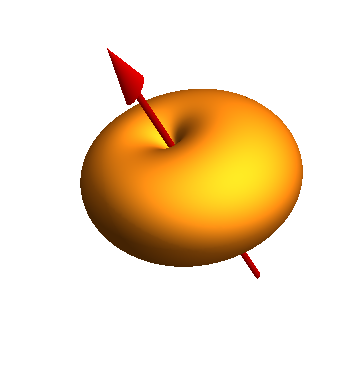
\includegraphics[width=0.525\textwidth]{gfx/Majorana/majorana_hole_low_res}}%
}
\caption{Walraven rethermalisation. I want to do this simulation for some different perturbation temperatures. One more higher and one lower too.}\label{fig:majorana_hole}
\end{figure}
In \autoref{fig:majorana_hole} we can see this surface looks like a disc that has been punctured either side along the axis of the trajectory of the atom.
This is because an atom that passes directly through the field minimum has a zero probability of making a non-adiabatic transition.
Of course this visualisation is only for a particular velocity, and since we have a thermal spread of velocities the average Majorana hole will look something more like the disc approximated by \autoref{eq:majorana_radius}.
So on average the approach taken in \autoref{sec:majorana_loss_rates} will be reasonably accurate however \autoref{eq:majorana_surface} may be more useful for a direct numerical approach.



